Un depósito es un cono circular invertido, de altura $6\,\mathrm m$ y radio superior $2.5\,\mathrm m$. El agua sale por un orificio circular de radio $0.02\,\mathrm m$ en el vértice inferior, con velocidad $0.6\sqrt{2gh}$, $g=9.8\,\mathrm{m/s^2}$. Determine la EDO para la altura de agua $h$.

Se supone líquido incompresible, salida única por el orificio, geometría cónica ideal y ley de salida suministrada. La EDO para la altura se usa mientras $h>0$; su coeficiente singular al agotarse el agua impide aplicarla literalmente en $h=0$.

\Needspace{11.28cm}
\begin{center}
\begin{minipage}{\linewidth}
\centering
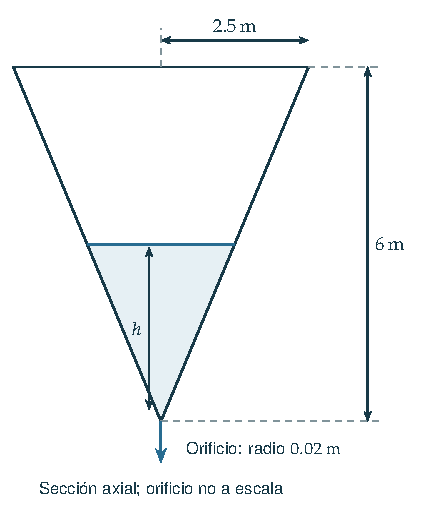
\includegraphics[width=8.03cm]{assets/M2-E0219-setup.pdf}\par
\smallskip{\small Geometría del depósito cónico y referencia de la altura de agua.\par}
\end{minipage}
\end{center}
